\documentclass[11pt]{article}

\usepackage{titlesec}
\usepackage[english]{babel}
\usepackage{parskip}
\usepackage{xcolor}
\usepackage{graphicx}
\graphicspath{ {./Images/} }
\usepackage{wrapfig}
\usepackage{array}
\usepackage{hyperref}
\hypersetup{
    colorlinks=true,
    linkcolor = white,
    urlcolor=cyan   
}

\urlstyle{same}

\titleformat{\section}[hang]{\Huge \bfseries \centering}{\thesection. }{0pt}{}{}
\titleformat{\subsection}[hang]{\Large \bfseries  }{\thesubsection. }{0pt}{}{}

\definecolor{background}{RGB}{54,57,63}
\pagecolor{background}
\color{white}

\begin{document}

\title{Tankfei Guide: Ace Protector \vfill 
\includegraphics[scale= 1.45 ]{YanfeiPixel.png} \vfill
}
\author{A Tankfei guide by Bonime\#0026}
\date{Updated for 3.1}
\maketitle
\newpage
\tableofcontents
\newpage 
\section{Preface}

Tankfei faces stiff competition from Diona, Thoma and Bennett. Therefore most players do not need to build Tankfei, and would be rewarded more building the other characters.

Therefore, I suspect that many who build Tankfei will build her for non-meta reasons (like me). I hope that by the end of the guide, you will fully understand Tankfei, and can get some ideas for teams to build. 

\section{Why play Tankfei} 

\subsection{Pros}

\textbf{Competitive cheap shield}

When correctly built, Tankfei sustain a shield comparable to well built Diona and Thoma, due to her 45\% Max HP shield scaling. 

\textbf{Pyro Swirl Enabler}

Tankfei can provide just enough pyro to overtake a strong hydro aura, enabling an anemo character to pyro VV shred and increase the team's damage output.

\textbf{Weapon Options}

Tankfei has access to both Prototype Amber and Thrilling Tales of Dragon Slayer, both providing strong utility for Tankfei's team.

\textbf{Low investment}

Tankfei has no need for raised talents, as her shield comes from constellations. Two of her weapons options are craftable, and her third option is a 3 star catalyst. 

4 Noblesse can be farmed using the artefact strongbox, meaning you can be building another character, and fodder bad artifacts for Tankfei. You can also go 2 Tenacity/2 Emblem if you have the resin or some free pieces.

Her heaviest costs are getting Tankfei to level 90, building enough \%ER to burst every rotation and getting an R5 Prototype Amber if needed. 

\subsection{Cons}

\textbf{80 Burst Cost / 20 Burst CD}

Tankfei's shield is completely locked behind her burst, which costs 80 energy. It's nearly impossible to run Tankfei without another pyro character. Tankfei's team also have to go with a 20 second rotation. Other shielders can opt for shorter rotations, either in their base kit or via constellations.

\textbf{Lacking Utility}

Tankfei's only utility is her shield. Other support often bring more to the table. Diona provides movement speed and stamina reduction, Bennett brings his ATK buff and even Thoma has his offield pyro application. 

\textbf{Outscaled}

Tankfei's shield can get outscaled by the other shielders if you heavily invest into talents, and collect constellations. However, Tankfei shield still remains a competitive option among 4 star shielders.



\section{Tankfei TLDR}

\begin{figure}[h]
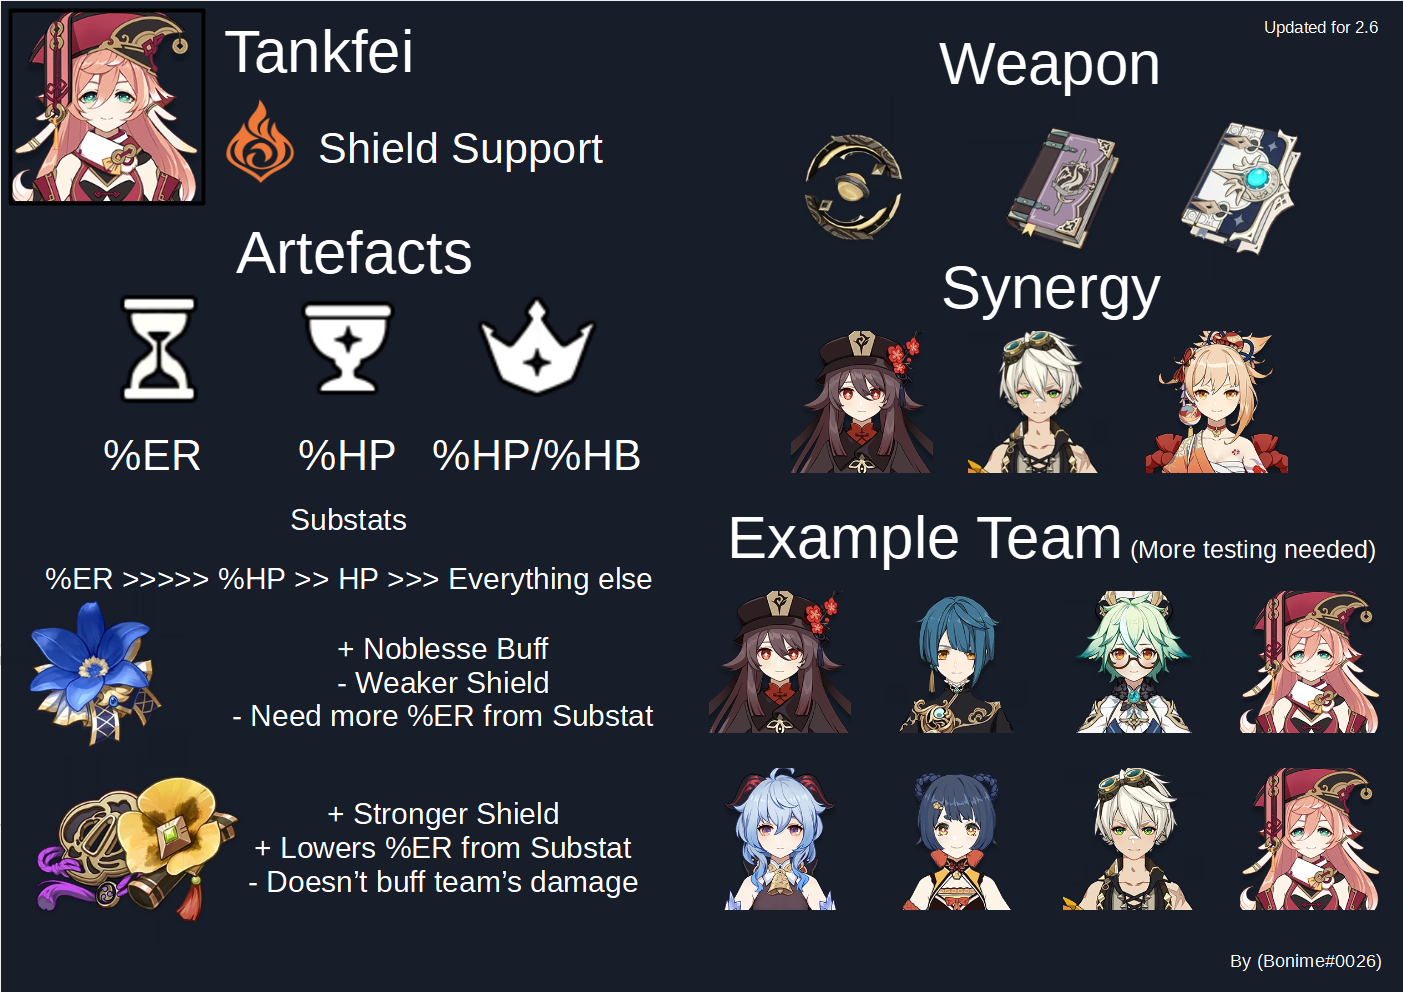
\includegraphics[scale= 0.235]{Tankfei.png} 
\centering
\end{figure}

\newpage

\section{Character Overview}

\subsection{Base Kit}

\begin{tabular}{m{0.1\textwidth} m{0.8\textwidth} }

\includegraphics[scale = 0.27]{NormalAttack.png}  & \textit{Tankfei's Normal Attack: Seal of Approval} 

You won't be auto attacking much on Tankfei. Charged attacks are only used to apply pyro for an anemo character.\\
\\

\includegraphics[scale = 0.27]{ElementalSkill.png} & \textit{Tankfei's Elemental Skill: Signed Edict} 

Signed Edict generates 3 pyro particles with a 9 second CD. Scarlet seals, generated by Signed Edict, increase the AoE and decrease the stamina cost of Tankfei's next charged attack. \\
\\

\includegraphics[scale = 0.27]{ElementalBurst.png} & \textit{Tankfei's Elemental Burst: Done Deal} 

Done Deal is how Tankfei generates her shield. It has an 80 energy cost and 20 second CD. Tankfei's biggest question is how can you secure her burst every rotation? \\
\\

\includegraphics[scale = 0.27]{Ascension1_Greyscale.png} & \textit{Tankfei's Ascension 1 Talent: Proviso} 

 Provides bonus \%Pyro DMG after landing a charged attack based off the number of scarlet seal consumed. This ascension passive is useless for Tankfei, as Tankfei is a quickswap support \\
 \\

\includegraphics[scale = 0.27]{Ascension4_Greyscale.png} & \textit{Tankfei's Ascension 4 Talent: Blazing Eye} 

Provides an extra instance of Pyro DMG after landing a crit charged attack on an opponent. This ascension passive is useless, as you are not building crit rate on Tankfei \\
\\

\includegraphics[scale = 0.27]{Passive.png} & \textit{Tankfei's Passive Talent: Encyclopedic Expertise} 

Shows Liyue unique resources on the map. One of the more useful passive. Makes building other Liyue characters easier. \\

\end{tabular}

\subsection{Talents and Levels}

Do not level your talents, since Tankfei's shield comes from her constellation. Getting Tankfei to level 90 is a priority to raise her low base HP. 

\subsection{Constellations}

Outside her 4$^{th}$ constellation, the others are either minor upgrades, or inconsequential. Let's have a look.

\begin{tabular}{m{0.1\textwidth} m{0.8\textwidth} }

\includegraphics[scale = 0.27]{Constellation1_Greyscale.png}  & \textit{Tankfei's 1$^{st}$ Constellation : The Law Knows No Kindness} 

Each Scarlet seal reduces charge attack stamina consumption by 10\% and increases resistance against interruption when released. Both are nice, but neither are necessary. \\
\\

\includegraphics[scale = 0.27]{Constellation2.png} & \textit{Tankfei's 2$^{nd}$ Constellation : Right of Final Interpretation} 
    
Increase charge attack crit rate by 20\% versus enemies below 50\% HP. Makes Favonius build a little less copium, but again not necessary \\
\\

\includegraphics[scale = 0.27]{Constellation3_Greyscale.png} & \textit{Tankfei's 3$^{rd}$ Constellation : Samadhi Fire-Forged} 
    
Increases Signed Edict Talent level by 3. Ignorable. The damage increase was already negligible for Yanfei, so it's worthless for Tankfei. \\
\\

\includegraphics[scale = 0.27]{Constellation4.png} & \textit{Tankfei's 4$^{th}$ Constellation : Supreme Amnesty} 
    
Generates a shield that lasts 15 seconds, based of 45\% of Tankfei's max HP, that absorbs pyro damage 250\% more efficiently. Tankfei signature constellation. A must for Tankfei. \\
\\

\includegraphics[scale = 0.27]{Constellation5_Greyscale.png} & \textit{Tankfei's 5$^{th}$ Constellation : Abiding Affidavit} 
    
Increases Done Deal Talent level by 3. Effective use of this constellation requires field time, which is not what we want for Tankfei.\\
\\

\includegraphics[scale = 0.27]{Constellation6.png} & \textit{Tankfei's 6$^{th}$ Constellation : Extra Clause} 
    
Maximum scarlet seal is increase to 4. With 4 scarlet seal, Tankfei can charged attack for no stamina cost after either her skill or burst. A nice but situational constellation.  \\
    
\end{tabular}

\newpage

\section{Playstyles}

We will focus on Tankfei as a support, as opposed to Tankfei as a main DPS. If you want to read more on how to make Tankfei into a main DPS (Yanfei), do check out the \href{https://keqingmains.com/yanfei/}{KQM Yanfei guide}.  

\subsection{General Principles}

Tankfei is a support character whose main purpose is to provide a shield every rotation. Since she contributes little to no damage, we aim to minimize the time she spends onfield. 

\subsection{Skill Order}

Tankfei has 2 main jobs. Create a shield using Done Deal (Q) and battery herself with Signed Edict (E). If necessary, Tankfei should apply pyro for swirl with her charged attack (C). Now, consider these three things.

1. Signed Edict particle's have travel time. We want to avoid using Signed Edict last, otherwise, we will need to wait for the particles to travel to us. 

2. Charge attacking is slow. We want to avoid charge attacking at all unless necessary, which mean only if we need to apply pyro for swirl. 

3. Scarlet seals from Signed Edict or Done Deal reduce the stamina cost of Tankfei's charged attack. Hence we want to avoid charge attacking first. 

Keeping all the above, and minimizing Tankfei onfield time, I came up with EQ, EQC and QEC. So when should each skill order be implemented? The flowchart below should help you choose the right skill order for you. 

\begin{center}
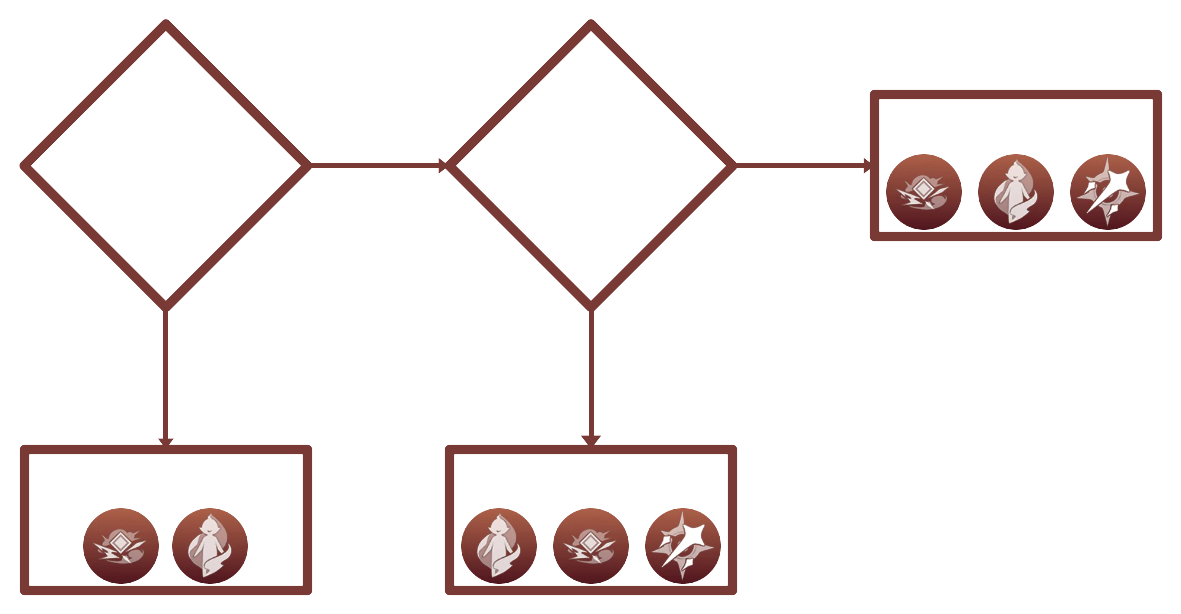
\includegraphics[scale = 0.2325]{Flowchart.png}
\end{center}

% EQ is for when Tankfei is used just for her shield. Whilst fast, it's also dangerous, since getting interrupted or switching out too fast can result in Tankfei not properly funnelling her Signed Edict's particles. 

% EQC is the optimal skill order for pyro application. Whilst slow and still interruptible, You do not need to wait for Signed Edict's particle, as they fly towards you during Done Deal and the charged attack. 

% QEC is the safe skill order for pyro application. Whilst slow, you are not interruptible, thanks to the shield. However, since you delayed Signed Edict, you must take care to not switch out too fast. 

\subsection{Double Signed Edict}

Tankfei team rotations are all 20 seconds longs, to line up with her Done Deal (Q) CD. But her Signed Edict (E) has a 9 second CD. One could use Signed Edict twice per rotation. This is what I call Double Signed Edict.

Tankfei does not need to collect both set of particles, so one set can be funnelled into another character. However, there are 2 main obstacles to doing Double Signed Edict.

1. In a 20 second rotation, you have 2 seconds where you can use another Signed Edict, and not extend the rotation itself. This is incredibly tight. 

2. Many main DPS characters have onfield time requirements lasting over 9 seconds. This makes it incredibly hard to fit 2 Signed Edicts per rotation. 

Extending the rotation solves the first problem, but this lowers both the teams DPS and Tankfei's shield uptime. The second problem is a character problem. It depends on how strict the onfield requirements are. 

Therefore, there are teams where double Signed Edicts is possible, and while it's an important tactic for Tankfei to know, in most teams you will not have access to this. 

\newpage

\section{Weapons}

\begin{tabular}{| m{0.13\textwidth}  | m{0.80\textwidth} |}
\hline Weapon & Name and Note \\
\hline  
\includegraphics[scale = 0.18]{WeaponPrototypeAmber.png}  & Prototype Amber: Tankfei's Best in slot. The \%HP makes her shield stronger and the passive alleviates her energy problems while making Tankfei into a team healer. \\
\hline  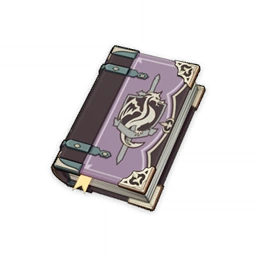
\includegraphics[scale = 0.18]{WeaponThrillingTalesofDragonSlayers.png}  & Thrilling Tales of Dragon Slayers (TTDS): A solid support catalyst. The \%HP makes her shield stronger and the passive adds to the teams damage, but it gives no energy for Tankfei. \\
\hline  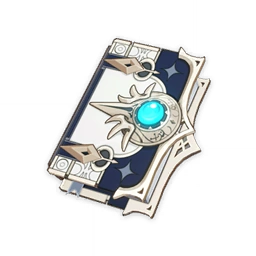
\includegraphics[scale = 0.18]{WeaponFavoniusCodex.png}  & Favonius Codex: \%ER catalyst. The \%ER makes this comparable to an R1 Prototype Amber without the healing. However, Tankfei struggles to activate the passive. \\
\hline  
\includegraphics[scale = 0.18]{WeaponFruitofFulfillment.png}  & Fruit of Fulfillment: A free to play alternative to Favonius Codex. Tankfei will not be making use of the passive at all. \\
\hline 
\end{tabular} 

In terms of ranking, based off flexibility (How easy it is to team build around each catalyst) and the catalyst's overall power level.

\begin{center}
Prototype Amber $>>>$ TTDS $>>>$  Favonius Codex $>>>$ Fruit of Fulfillment
\end{center}

Here is a list of other weapons I considered, but ended up not recommending.

- \textit{Sacrificial Fragment}: While being able to use two elemental skill per rotation is nice, it's passive is never consistent, making it a gamble if you can activate Tankfei's shield next rotation. 

- \textit{Oathswrown Eye}: You have to Double Signed Edict every rotation to even make this comparable to Favonius Codex, and Double Signed Edict are hard to pull off in most teams. 

- \textit{Wine and Song / Hakushin Ring / Otherworldly Story}: Not enough \%ER to justify using these over Favonius Codex. Hakushin passive is decent, but the low \%ER makes it not competitive.

\newpage 

\section{Artifacts}

\subsection{Artefact Main Stats}

The sands should always be \%ER. Tankfei needs a lot of \%ER rolls to help with her energy issues. Using a \%HP sands requires artifacts with higher \%ER substats, which is not a guarantee. 

The Goblet should always be \%HP, as there are no other options Tankfei can make good use of.

Circlet we have the options between \%HP and \%HB (\% Healing Bonus).

\begin{tabular}{|m{0.13\textwidth}|m{0.8\textwidth}|}
\hline Circlet  & Note \\ 
\hline \%HP & Adds a nice chunk of health onto Tankfei's shield. Since there are no \%ER option here, this becomes the main option. A generally excellent and solid option. \\
\hline \%HB & If you face units that deal damage through shields, \%HB can add 4$\sim$6 \% (Based on Refinements) Max HP on Prototype Amber's healing passive A situational option. \\
\hline
\end{tabular}

\subsection{Artefact Substat}

\begin{center}
    \%ER $>>>>>>$ \%HP $>>$ HP $>>>>>>$ Everything else
\end{center} Tankfei has one of the lowest base HP, making \%HP rolls worse. Moreover, her shield relies on Done Deal being activated, making \%ER rolls important.

To see recommended \%ER for Tankfei, see \textbf{Team Compositions}. Tankfei's \%ER requirements will depend heavily on what teammates she has, but aim for 230\%ER.

\textbf{My recommended \%ER assume enemies drop no particles and team generates all their particles}. Build what is recommended, as not having enough energy screws up Tankfei. Build more if necessary.  

Running solely on a fully levelled \%ER$\backslash$\%HP$\backslash$\%HP build, a level 90 Tankfei can pump a shield with just over 10,000 damage absorption. This is before weapons, substats and artefact sets bonuses are considered.  

So prioritizing \%ER isn't so bad, as her base shield is already quite high. All you need is to get the \%ER rolls to get to the recommended amount of \%ER.

\subsection{Artefact Set}

\begin{tabular}{|m{0.13\textwidth}  | m{0.80\textwidth} | }
\hline Set & Note \\
\hline \includegraphics*[scale = 0.51]{4NoblesseOblige - Copy2.png} & 4 Noblesse Oblige (4NO): Compress another role into Tankfei as the Noblesse holder. Since Noblesse however, does not help you with \%ER, you will need more \%ER rolls from substats \\
\hline \includegraphics*[scale = 0.69]{2Ten2Emblem.png} & 2 Tenacity of the Millileth / 2 Emblem of Severed Fate (2ToM/ 2EoSF): If your team bad synergy with 4NO, this combo will help Tankfei's shield and her \%ER issues.\\
\hline 
\end{tabular}

If you are going for the 2ToM / 2EoSF sets, then I recommend you farm the 2 ToM pieces first, till you have two good pieces. (15$\sim$20\%ER on both artifacts, or an \%ER sands and 15$\sim$20\%ER on the other artefact). 

This does makes it harder to get the remaining Emblem pieces, but staying in the Emblem domain is not a bad idea, as the Emblem artefact set is used by many other support characters. 

If you have none of the above options, 2 Emblem with 3 high \%ER pieces is the way to go. If you are below AR45, and planning to build Tankfei, I'd recommend you wait, simply because of the high \%ER requirements.

Here is a list of other artefact sets I considered, but ended up not recommending.

\textit{2 \%HB set bonus:} Trading in 20\% ER , 20\% HP or 4NO passive for slightly more healing isn't worth it in most situations.  

\textit{4 Maiden Beloved:} Similar shield strength to a 4NO build, but you only improve Tankfei's healing. Generally not worth 

\textit{4 Ocean Hued Clam:} The added damage from the 4 Ocean Hued Clam passive does not justify using 4 Ocean Hued Clam over 4 Noblesse Oblige.  

\textit{4 Instructors:} Yanfei relies too much on \%ER and \%HP substats to competitively run 4 Instructor. If you could run Instructor, you would run TTDS instead. 



\newpage 

\section{Team Compositions}

Because of Tankfei's energy problems, you are often going to run another pyro character in the team to help Tankfei with her energy issues. From the current pool of pyro characters, we can remove some options

\begin{figure}[h]
    \centering
    
\includegraphics[scale = 0.25]{Character_Amber.png}
    
\includegraphics[scale = 0.25]{Character_Thoma.png}
    
\includegraphics[scale = 0.25]{Character_Xinyan.png}
\end{figure}

\textit{Amber, Thoma, Xinyan:} All 3 options compete with Tankfei in some manner. Thoma and Xinyan shield, and all 3 output similar or faster pyro application. 

\begin{figure}[h]
    \centering
    
\includegraphics[scale = 0.25]{Character_Diluc.png}
    
\includegraphics[scale = 0.25]{Character_Klee.png}
    
\includegraphics[scale = 0.25]{Character_Xiangling.png}
\end{figure}

\textit{Diluc, Klee, Xiangling:} These characters would rather have Bennett than Tankfei. And Bennett is an extremely strong character, so I am not going to advise using Tankfei as a replacement.

This leaves us with 3 options. Hu Tao, Yoimiya and Bennett. Since Tankfei lacks any sort of \% Shield strength, it is reccomended that Yoimiya goes 4 Retracing Bolide when Tankfei runs 4 Noblesse. 

\newpage 

\subsection{Hu Tao Teams}

\textbf{VV Vape Hu Tao}

\begin{center}
    \begin{tabular}{m{0.21\textwidth} m{0.21\textwidth} m{0.21\textwidth} m{0.21\textwidth}}
        
\includegraphics[scale = 0.25]{Character_Hu_Tao.png}  & 
\includegraphics[scale = 0.25]{Character_Xingqiu.png} &
\includegraphics[scale = 0.19]{Element_Anemo.png} &  
\includegraphics[scale = 0.25]{Character_Yanfei.png} \\
    \end{tabular}
\end{center}

Where the Anemo option can be Kazuha or Sucrose

\textbf{\small{Build}}

Weapon: Prototype Amber or Favonius Codex / Fruit of Fulfillment 

Artefact Set: 2 EoSF / 2 ToM

Main Stat: \%ER/\%HP/\%HP 

\begin{tabular}{m{0.08\textwidth} m{0.8\textwidth}}
    \%ER: & Favonius Codex / Fruit of Fulfillment: 300\% to 270\% \\
    & R1 Prototype Amber: 250\% to 230\% \\
\end{tabular}

\textbf{\small{Rotation}} 

For rotations, see the VV vape section page on the \href{https://keqingmains.com/hu-tao/}{KQM Hu Tao guide}. They have nice videos and cover both anemo options. For Tankfei, do EQC or QEC for the pyro application.

\textbf{\small{- Pros}}

\begin{itemize}
    \item Great single target damage
    \item Access to shields and pyro resonance via Tankfei
    \item Double VV shred is available 
\end{itemize}

\textbf{\small{- Cons}}

\begin{itemize}
    \item Difficult team to operate 
    \item Lacking in the AoE department
    \item Very high \%ER requirements 
    \item Requires Xingqiu, a highly demanded unit 
\end{itemize}

\newpage

\subsection{Yoimiya Teams}

\textbf{Overvape Yoimiya Team}

\begin{center}
    \begin{tabular}{m{0.21\textwidth} m{0.21\textwidth} m{0.21\textwidth} m{0.21\textwidth}}
        
\includegraphics[scale = 0.25]{Character_Yoimiya.png}  & 
\includegraphics[scale = 0.25]{Character_Yelan.png} &  
\includegraphics[scale = 0.25]{Character_Fischl.png} & 
\includegraphics[scale = 0.25]{Character_Yanfei.png}\\
    \end{tabular}
\end{center}

\textbf{\small{Build}}

Weapon: Prototype Amber

Artefact Set: 4NO or 2 EoSF / 2 ToM

Main Stat: \%ER/\%HP/\%HP or \%ER/\%HP/\%HB

\%ER: R5 Prototype Amber: 230\% to 210\%

\textbf{\small{Rotation}} 

\begin{center}
    Yelan EQ $>>$ Tankfei EQ $>>$ Fischl E or Q $>>$ Yoimiya E N5$\times$3 
\end{center}

\textbf{\small{- Pros}}

\begin{itemize}
    \item Great single target damage
    \item Access to heals, shields and pyro resonance via Tankfei
    \item Easy to pilot
\end{itemize}

\textbf{\small{- Cons}}

\begin{itemize}
    \item Lack of AoE damage 
    \item Yoimiya is not bursting every rotation
    \item Oz gives less damage if enemy moves too far away. 
    \item Requires Fischl, a highly demanded unit. 
\end{itemize}

\newpage
\textbf{VV Vape Yoimiya}

\begin{center}
    \begin{tabular}{m{0.21\textwidth} m{0.21\textwidth} m{0.21\textwidth} m{0.21\textwidth}}
        
\includegraphics[scale = 0.25]{Character_Yoimiya.png}  & 
\includegraphics[scale = 0.25]{Character_Yelan.png} &
\includegraphics[scale = 0.19]{Element_Anemo.png} &  
\includegraphics[scale = 0.25]{Character_Yanfei.png} \\
    \end{tabular}
\end{center}

Where the Anemo option can be Kazuha or Sucrose

\textbf{\small{Build}}

Weapon: Prototype Amber

Artefact Set: 2EoSF / 2ToM or 4NO

Main Stat: \%ER/\%HP/\%HP 

\%ER: R5 Prototype Amber: 240\% to 220\%

\textbf{\small{Rotation}} 

\begin{center}
    Yelan EQ $>>$ Tankfei EQC $>>$ Sucrose N2E $>>$ Yoimiya QE N5$\times$3
\end{center}
\begin{center}
    Yelan EQ $>>$ Tankfei EQC $>>$ Kauzha EEQ $>>$ Yoimiya QE N5$\times$3
\end{center}

\textbf{\small{- Pros}}

\begin{itemize}
    \item Great single target damage
    \item Access to shields, heals and pyro resonance via Tankfei
    \item Double VV shred is available 
\end{itemize}

\textbf{\small{- Cons}}

\begin{itemize}
    \item Difficult team to operate
    \item Yoimiya is not bursting every rotation
    \item Lacking in the AoE department
    \item Sucrose low particle generation hurts Tankfei
\end{itemize}

\newpage

\textbf{Vape Yoimiya Team}

\begin{center}
    \begin{tabular}{m{0.21\textwidth} m{0.21\textwidth} m{0.21\textwidth} m{0.21\textwidth}}
        
\includegraphics[scale = 0.25]{Character_Yoimiya.png}  & 
\includegraphics[scale = 0.25]{Character_Yelan.png} &  
\includegraphics[scale = 0.25]{Character_Yun_Jin.png} & 
\includegraphics[scale = 0.25]{Character_Yanfei.png}\\
    \end{tabular}
\end{center} 

\begin{center}
    \begin{tabular}{m{0.21\textwidth} m{0.21\textwidth} m{0.21\textwidth} m{0.21\textwidth}}
        
\includegraphics[scale = 0.25]{Character_Yoimiya.png}  & 
\includegraphics[scale = 0.25]{Character_Yelan.png} &  
\includegraphics[scale = 0.25]{Character_Candace.png} & 
\includegraphics[scale = 0.25]{Character_Yanfei.png}\\
    \end{tabular}
\end{center}

\textbf{\small{Build}}

Weapon: Prototype Amber

Artefact Set: 2EoSF / 2ToM or 4NO

Main Stat: \%ER/\%HP/\%HP or \%ER/\%HP/\%HB

\%ER: R5 Prototype Amber: 230\% to 210\%

\textbf{\small{Rotation}} 

\begin{center}
    Yelan EQ $>>$ Tankfei EQ $>>$ YunJin EQ $>>$ Yoimiya QE N5$\times$3
\end{center}
\begin{center}
    Yelan EQ $>>$ Tankfei EQ $>>$ Candace EQ $>>$ Yoimiya QE N5$\times$3
\end{center}

\textbf{\small{- Pros}}

\begin{itemize}
    \item Great single target damage
    \item Access to heals, shields and pyro resonance via Tankfei
    \item Normal attack buffs are strong on Yoimiya
\end{itemize}

\textbf{\small{- Cons}}

\begin{itemize}
    \item Lack of AoE damage 
    \item Yoimiya is not bursting every rotation
    \item Requires investment into multiple units
    \item YunJin/Candace need to be on a Favonius weapon
\end{itemize}

\newpage 

\subsection{Bennett Teams}

\textbf{Melt Ganyu}

\begin{center}
    \begin{tabular}{m{0.21\textwidth} m{0.21\textwidth} m{0.21\textwidth} m{0.21\textwidth}}
        
\includegraphics[scale = 0.25]{Character_Ganyu.png}  & 
\includegraphics[scale = 0.25]{Character_Xiangling.png} &  
\includegraphics[scale = 0.25]{Character_Bennett.png} & 
\includegraphics[scale = 0.25]{Character_Yanfei.png}\\
    \end{tabular}
\end{center}

\textbf{\small{Build}}

Weapon: Prototype Amber 

Artefact Set: 2EoSF / 2ToM 

Main Stat: \%ER/\%HP/\%HP 

\%ER: R5 Prototype Amber: 220\% to 200\%

\textbf{\small{Rotation}} 

\begin{center}
    Yanfei EQ $>>>$ Bennett QE $>>>$ Xiangling (E)Q $>>>$ Ganyu C5 E $>>>$ Bennett E $>>>$ Xiangling E
\end{center} 
\begin{center} 
    Where Xiangling should EQ on the first rotation. After that, Xiangling should just Q. 
\end{center}

\textbf{\small{- Pros}}

\begin{itemize}
    \item Lots of AoE and Single Target damage
    \item Access shields and pyro resonance via Tankfei
    \item Xiangling, Bennett and Tankfei help each other's energy
\end{itemize}

\textbf{\small{- Cons}}

\begin{itemize}
    \item Xiangling and Tankfei bring energy issues.
    \item Requires investment into multiple units
\end{itemize}

\newpage

\textbf{XiaoDen}

\begin{center}
    \begin{tabular}{m{0.21\textwidth} m{0.21\textwidth} m{0.21\textwidth} m{0.21\textwidth}}
        
\includegraphics[scale = 0.25]{Character_Xiao.png}  & \includegraphics[scale = 0.25]{Character_Raiden_Shogun.png} &  \includegraphics[scale = 0.25]{Character_Bennett.png} & \includegraphics[scale = 0.25]{Character_Yanfei.png}\\
    \end{tabular}
\end{center} 

\textbf{\small{Build}}

Weapon: Thrilling Tales of Dragon Slayers

Artefact Set: 2 EoSF / 2 ToM 

Main Stat: \%ER/\%HP/\%HP 

\%ER: Thrilling Tales of Dragon Slayers: 230\% to 220\%

\textbf{\small{Rotation}} 

\begin{center}
    Raiden E $>>>$ Bennett EQ $>>>$ Yanfei EQ $>>>$ Xiao E2Q $>>>$ Raiden EQ
\end{center} 

\textbf{\small{- Pros}}

\begin{itemize}
    \item Team has access to single target and AoE damage
    \item Tankfei high burst cost help Raiden damage. 
    \item Raiden helps Tankfei's energy problems. 
    \item Access shields and pyro resonance via Tankfei
\end{itemize}

\textbf{\small{- Cons}}

\begin{itemize}
    \item Buffs cannot be given to both Xiao and Raiden
    \item Xiao and Tankfei depend on Raiden for Energy 
\end{itemize}

\newpage 

\textbf{Tankfire Barbara}

\begin{center}
    \begin{tabular}{m{0.21\textwidth} m{0.21\textwidth} m{0.21\textwidth} m{0.21\textwidth}}
        \includegraphics[scale = 0.25]{Character_Barbara.png}  & \includegraphics[scale = 0.25]{Character_Jean.png} &  \includegraphics[scale = 0.25]{Character_Bennett.png} & \includegraphics[scale = 0.25]{Character_Yanfei.png}\\
    \end{tabular}
\end{center} 

\textbf{\small{Build}}

Weapon: Thrilling Tales of Dragon Slayers

Artefact Set: 2 EoSF / 2 ToM

Main Stat: \%ER/\%HP/\%HP 

\%ER: Thrilling Tales of Dragon Slayers: 250\%

\textbf{\small{Rotation}} 

\begin{center}
    Bennett Q $>>>$ Tankfei Q $>>>$ (Barbara C) $>>>$ Jean Q $>>>$ Barbara C4 $>>>$ Jean EN3 $>>>$ Bennett E $>>>$ Tankfei E $>>>$ Barbara C $>>>$ Jean E
\end{center} 

\textbf{\small{- Pros}}

\begin{itemize}
    \item Good Single Target and AoE damage. 
    \item Access shields and pyro resonance via Tankfei
\end{itemize}

\textbf{\small{- Cons}}

\begin{itemize}
    \item Barbara not generating energy is detrimental to Tankfei's energy.
    \item Jean needs to carry Favonius Sword
\end{itemize}

\newpage

\textbf{Vape Barbara}

\begin{center}
    \begin{tabular}{m{0.21\textwidth} m{0.21\textwidth} m{0.21\textwidth} m{0.21\textwidth}}
        \includegraphics[scale = 0.25]{Character_Barbara.png}  & \includegraphics[scale = 0.25]{Character_Bennett.png} &  \includegraphics[scale = 0.25]{Character_Xiangling.png} & \includegraphics[scale = 0.25]{Character_Yanfei.png}\\
    \end{tabular}
\end{center} 

\textbf{\small{Build}}

Weapon: Prototype Amber 

Artefact Set: 2EoSF / 2ToM 

Main Stat: \%ER/\%HP/\%HP 

\%ER: R5 Prototype Amber: 230\% to 220\%

\begin{center}
    Yanfei EQ $>>>$ Bennett QE $>>>$ Xiangling (E)Q $>>>$ Barbara C4 $>>>$ Bennett E $>>>$ Xiangling EN3
\end{center} 
\begin{center} 
    Where Xiangling should EQ on the first rotation. After that, Xiangling should just Q. 
\end{center}

\textbf{\small{- Pros}}

\begin{itemize}
    \item Good Single Target and AoE damage. 
    \item Access shields and pyro resonance via Tankfei
\end{itemize}

\textbf{\small{- Cons}}

\begin{itemize}
    \item Barbara not generating energy is detrimental to Tankfei's energy.
    \item Xiangling needs to carry Favonius Lance
\end{itemize}

\newpage

\section{Acknowledgements}

Hu Tao Mains 

\begin{itemize}
    \item Popularizing Tankfei
\end{itemize}

\href{https://docs.google.com/document/d/15Fagrd1OD6fvgj0PEZKkbwiRmivgMd_MZZN_rcb8ZBE/edit#}{Xiaoden Theory Crafters}
\begin{itemize}
    \item Showing us Xiaoden
    \item Putting Build, Rotation, Pros and Cons
\end{itemize}

\href{https://www.youtube.com/c/furu212}{Youtube Channel Furu}

\begin{itemize}
    \item Showing us Tankfire Barbara
    \item Putting Build, Rotation, Pros and Cons
    \item Completing 3 abysses with the team (2.6 , 2.7, 2.8)
\end{itemize}

Chronopolize\#6513 from CoY Discord Server

\begin{itemize}
    \item Showing me Melt Ganyu
    \item Putting Rotation
    \item Completing Aybss with Melt Ganyu (2.8)
\end{itemize}




\end{document}
